% Chapter 6
\chapter{Advertisement High Fidelity prototype} % Main chapter title

\label{Chapter6} % For referencing the chapter elsewhere, use \ref{Chapter1} 

\newpage

\section{Introduction}


Various studies are conducted in different stages of a research, at this level the chapter concentrates to Experimental study, which is mostly done in a controlled environment or even at fields and finds variable that causes of a direct influence on another variable, there have been many Experimental studies like ``\emph{Sweep and point \& shoot}'' \cite{SweepPointShoot} that evaluated prototypes of interaction of personal computing device with large public displays, another was an evaluation of ``\emph{mobile interaction with live video}'' \cite{TouchProjector} in that the participants performance were measured for automatic zooming and temporary image freezing, which was an experimental with-in subject study design. Sebastian .D \cite{WalldragandDrop} assessed the general performance of drag and drop interaction on large displays and compared it with a traditional drag and drop. Jorg Müller \cite{LookingGlass} did pre-studies (lab and field) on noticing interactivity of a display in which the time required for recognizing interactivity by participants were measured.

After low-fi prototype evaluation and refining the prototype, the Hi- fidelity prototype version of advertisement got ready and this chapter explains the steps taken for advertisement application evaluation. The focus of this study were more on user performance like task completion time and call-to-action \cite{call-to-action} understandability, it also investigated on user acceptance that how much the interaction techniques were motivated for them and if they would interact in future, it also focused on the possible usability issues of the techniques.

This usability testing was to understand whether both mobile and body interactive advertisement would function in the public or not, what were other difficulties, confusions, common mistakes, and behavior toward the applications. As the application would be in public crowd and not just one person would pass by the screen we were also interested that how the application deal with many users while interacting and observe multi user behavior in front of the screen.


\section{Research questions}

In this part of the study the bellow research questions should be answered after the study is conducted. 

\subsection{Body and Mobile interactions}
\begin{enumerate}
\item	How fast do users understand call-to-action?
\item	How fast participants react to the call-to-action?
\item	How easy participants understand the interaction task?
\item	How long participants take to finish the interaction or visit all target locations?
\item	What are the major usability flaws that prevent users from advertisement interactions?
\item	What is the difference between mobile and body performance.
\item   How the applications would perform in one user interaction and in multi user interaction?
\end{enumerate}

\subsection{Video advertisement}
\begin{enumerate}
\item	Do participants understand about the content of advertisement?
\item	How many elements of display can participants recall after their first interaction?
\end{enumerate}


\section{Test Design}
Within-Subject Design was chosen, in this test participants were asked to experience with both Body and Mobile Interactions, The interaction sequences were vary for participants in order to counterbalance to be able to limit the effects of learning transfer. 

\subsection {Participants}
12 participants were invited for the usability testing; from which five participants were female and seven were male, most of the participants had computer science background and were familiar with mobile and had seen or worked with body sensing technologies, one participant was not familiar with QR-code.

\subsection{Task}
Participants were not told about any specific task, they were told to explore the system by their own and understand what to do, To avoid different outcomes participants were told to continue interaction until they encounter the very first stage of the application. So the tasks for participants were to start from initial stage of the interaction (body /mobile) and continue until reach again the initial stage.

As for body interaction no extra device was required to accomplish the task, but for mobile interaction a mobile phone was required, Participants were not told that the use of mobile is required unless participants used their own phone or asked for it from us.

\subsubsection{call-to-action understandability}
To determine this, the participants will be asked to approach the screen and perform what is relevant as soon as possible, The participants will not be told that the screen would ask them to do something, The participants should understand the task by the call-to-action method used in both interaction methods. The duration from approaching to screen and triggering the game would be considered as time taken to understand call-to-action. 

Body interaction application can count how long does it take for the user to trigger the game, but for mobile interaction there is no pre-counting for each individuals because mobile users and Kinect camera are two separate technologies that is very hard to know which user hold the phone, therefor we used manual timer and asked the participant to think-aloud anything he understood about the task.

\subsubsection{Task understandability}
Participants should think aloud that what they will do after reading the task. 

\subsubsection{Task completion time}
Task completion time is measured from the time game starts until the game ends. 

\subsubsection{Content of Advertisement}
To check if the users understand the content of advertisement while interacting and while advertisement was shown, participants will be given paper and pen to write down words that they could recall from entire session.

\subsubsection{Usability issues}
Each participant was given five minutes to interact with advertisement after one another and questions were asked regarding the issues they faced.
The usability issues are all observed by the moderator at the scene and later while watching the recorded videos. To understand better each interaction is separately listed as bellow.

Anything, which was confusing and unclear for the participants, committed errors and misunderstood events, which were done by participants, will also be counted as a usability issue. 

\subsubsection{Data Gathering }
The bellow data were gathered.

\subsection{Performance data}
The bellow is the performance measures data that will be gathered after successful conduction of the test.
\begin{enumerate}
\item	Duration of call-to-action understandability.
\item	Duration of the reaction to call-to-action
\item	Task completion time.
\item	Count of usability issues.
\end{enumerate}
 
Each individual's performance with both mobile and body interactions was created in bar chart, this data could also be used to check for efficiency of the interactions techniques too.
 
Mean time value for call-to-action understandability, game triggering, task completion and whole interaction time was computed for each interaction techniques. Along the mean time the confidence interval was also taken in consideration.

\subsection{Preference data}
The preference data, which is the measures of participant opinion or thought process, like the think-aloud each participant performed, or the answers for the interviews and their feedbacks.

\subsection{Think aloud quotes}
Think-Aloud quotes were noted during the video observation, these quotes were important to check at which point in time users understand about the interaction and tasks. It also helped to analyze their reaction and feedbacks toward the tasks being done.

\subsection{Interview transcripts}
All the interviews were transcribed and color-coding technique was applied to analyze and comprehend different aspects and categories from the defined questions.
\hilight{attach the color code chart}


\subsection{Recordings}
There were two different recordings done during the session, first was video recording using camera at the backside that could record user actions and computer screen, the second recording was the screen recording of the application using QuickTime screen recorder. These recordings were used to analyze behavior, application performance and listen to the things participants said during interaction.


\begin{figure}[H]
    \centering
    \begin{subfigure}[H]{0.45\textwidth}
        \centering
        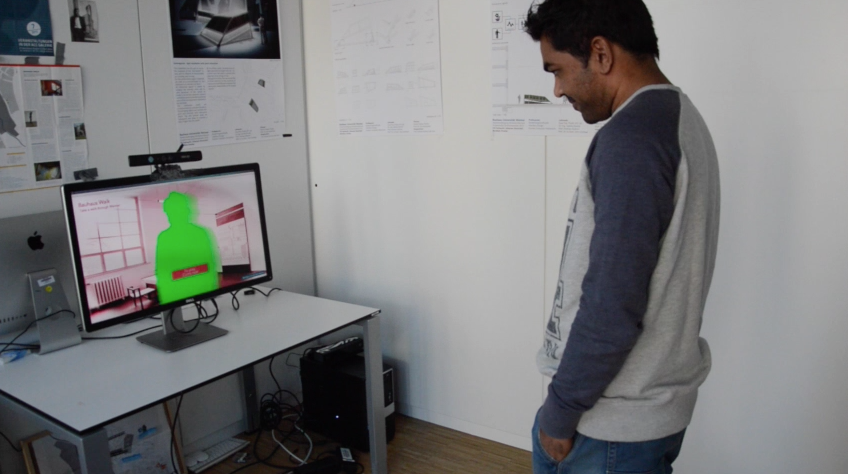
\includegraphics[width=\textwidth,height=4cm]{Figures/6/singleBody}
        \caption{Participant in body interaction mode.}
        \label{fig:singlebody}
    \end{subfigure}
    \hfill
    \begin{subfigure}[H]{0.45\textwidth}
        \centering
        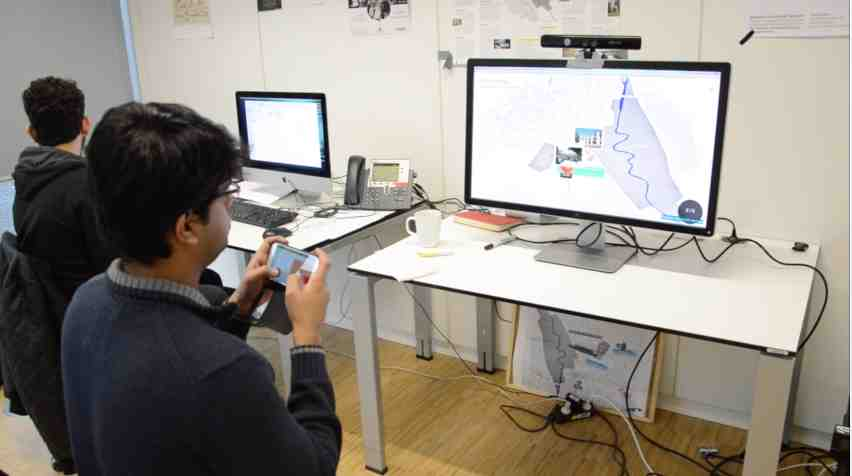
\includegraphics[width=\textwidth,height=4cm]{Figures/6/singleMobile}
        \caption{Participant in mobile interaction mode}
        \label{fig:singleMobile}
    \end{subfigure}
    \caption{}
    \label{fig:Focus_group_room}
\end{figure}


\section{Findings}

\subsection{Mobile Interaction performance}
The bellow chart shows four different aspects when the mobile interaction happened for participants. The y-axis shows duration in seconds and x-axis shows the aspects as bellow. You can see performance chart for each individual in Appedix \hilight{put number}
\begin{itemize}
\item Understand call-to-action,
\item Trigger game time
\item Understand task time
\item Game time.
\end{itemize}

\begin{figure}[H]
\centering
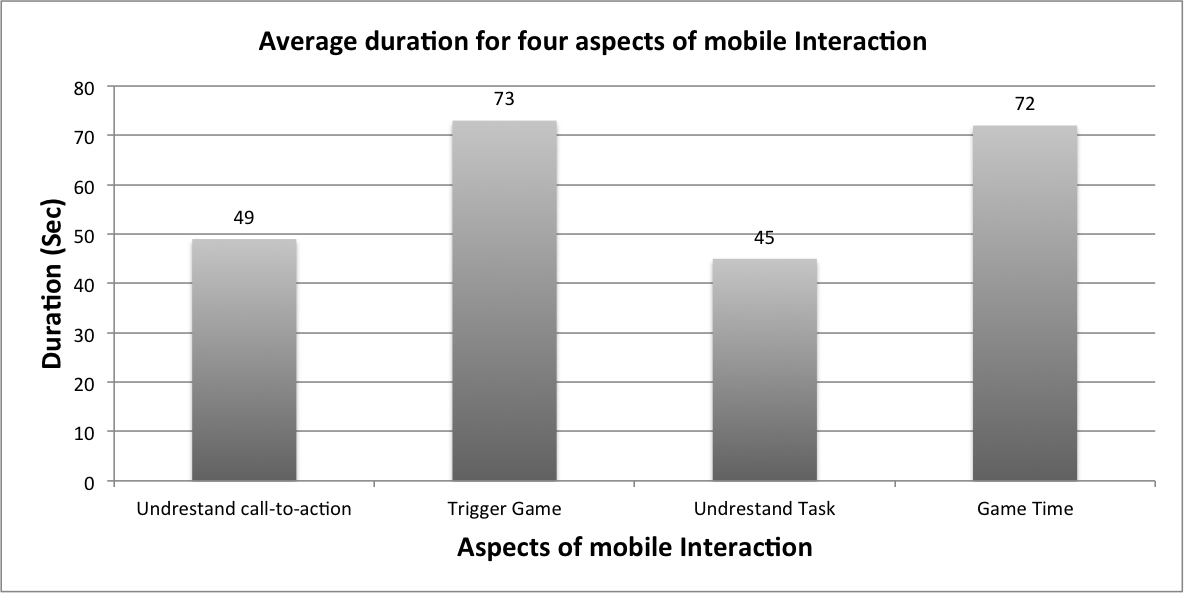
\includegraphics[width=12cm,height=5cm]{Figures/6/mobile_average}%
 \caption{Chart that shows each aspect with respect to duration. }%
 \label{fig:mobile_average}%
\end{figure}

As can be seen above participants took longer time approximately 240 seconds for whole interaction time. Participants took 49 seconds in average to understand how to access the system (call-to-action), After participants understood what to do it took 73 seconds in average from taking their phone, opening the web page, logging and starting the game, it took 45 seconds in average to figure out how to do the task and 72 seconds to complete the task.

%
%\begin{figure}[H]
%\centering
%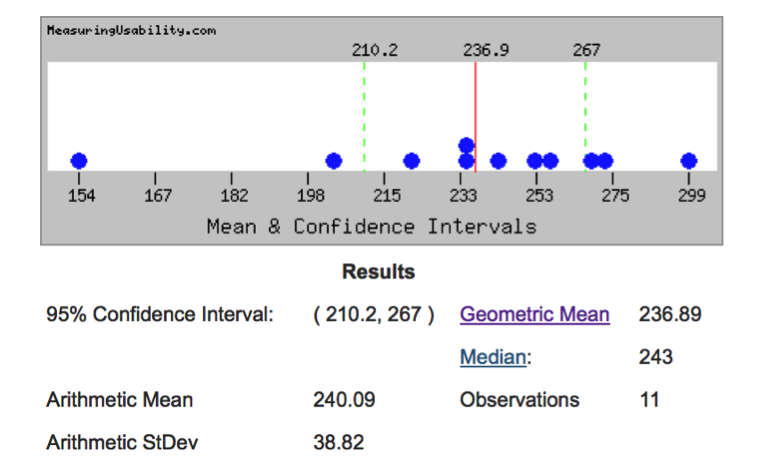
\includegraphics[width=12cm,height=6cm]{Figures/6/mobile_mean}%
% \caption{Confidence interval for Mobile interaction all phases duration }%
% \label{fig:mobile_mean}%
%\end{figure}

%above chart is generated in an online tool [1] with a confidence interval up to 95\% for complete interaction time for all 11 participants; the confidence interval is between (210.2, 267) the chart shows the Arithmetic standard deviation to be up to 38.82 seconds, Arithmetic Mean to be 240 seconds

\subsection{Body Interaction performance}
This also shows four different aspects of the body interaction in the bellow chart. To see all participant's interaction see Appendix. \hilight{put number}

\begin{figure}[H]
\centering
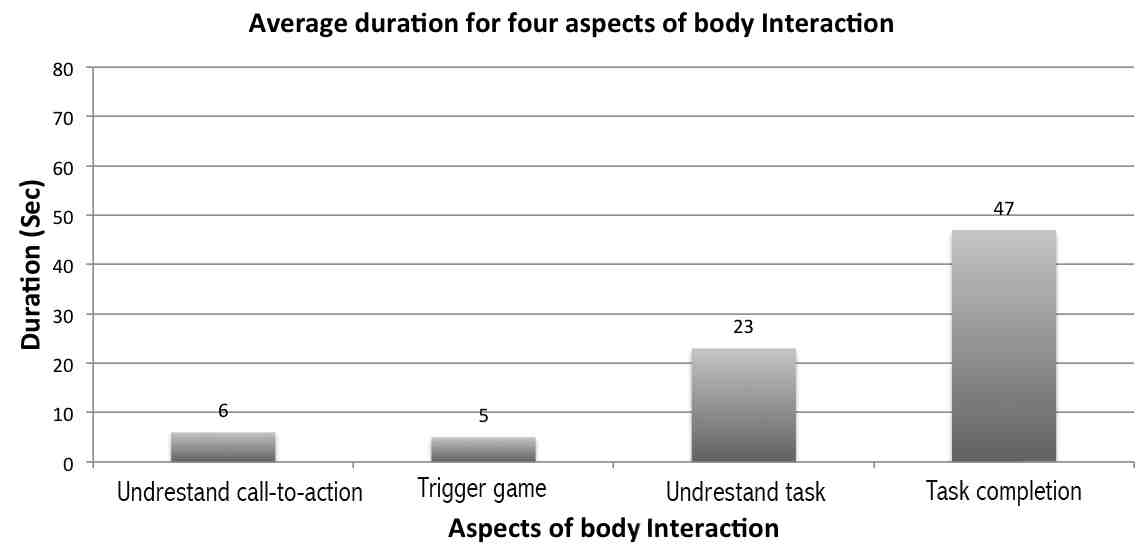
\includegraphics[width=12cm,height=5cm]{Figures/6/body_average}%
 \caption{Chart that shows each aspect with respect to duration}%
 \label{fig:body_average}%
\end{figure}

As can be seen above most of the participants finished the whole interaction in approximately 81 seconds, which is much better than mobile interaction. It took 6 seconds to understand call-to-action, 5 seconds to trigger and start the game, 23 seconds to understand the task and 47 seconds to complete the tasks.

%\begin{figure}[H]
%\centering
%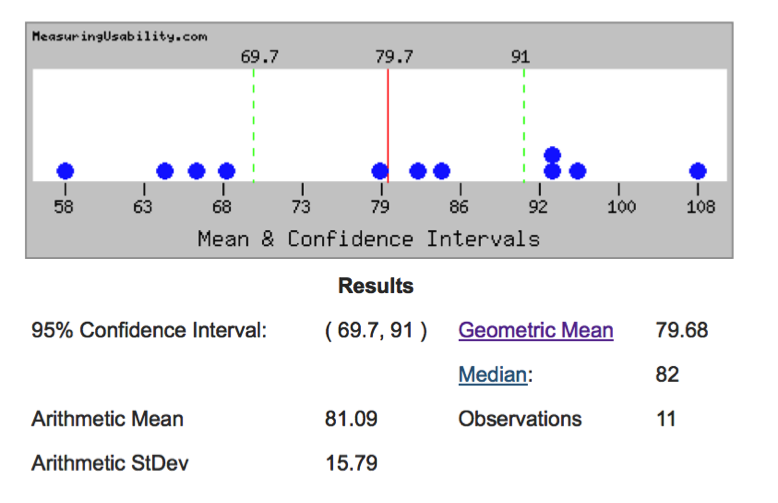
\includegraphics[width=12cm,height=6cm]{Figures/6/body_mean}%
% \caption{Confidence interval for body interaction all phases duration }%
% \label{fig:body_mean}%
%\end{figure}

%The above confidence interval for body interaction is generated using the web tool [1] for whole body interaction time. In which with the confidence interval of 95\% is between (69.7 ? 91) seconds, with the standard deviation of 15.79 seconds.


\subsection{Body Vs. Mobile performance}
As can be seen bellow body interaction seems to be much better than mobile interaction in terms of performance. The whole interaction time of body is less than the half of the time of mobile interaction. 

\begin{figure}[H]
\centering
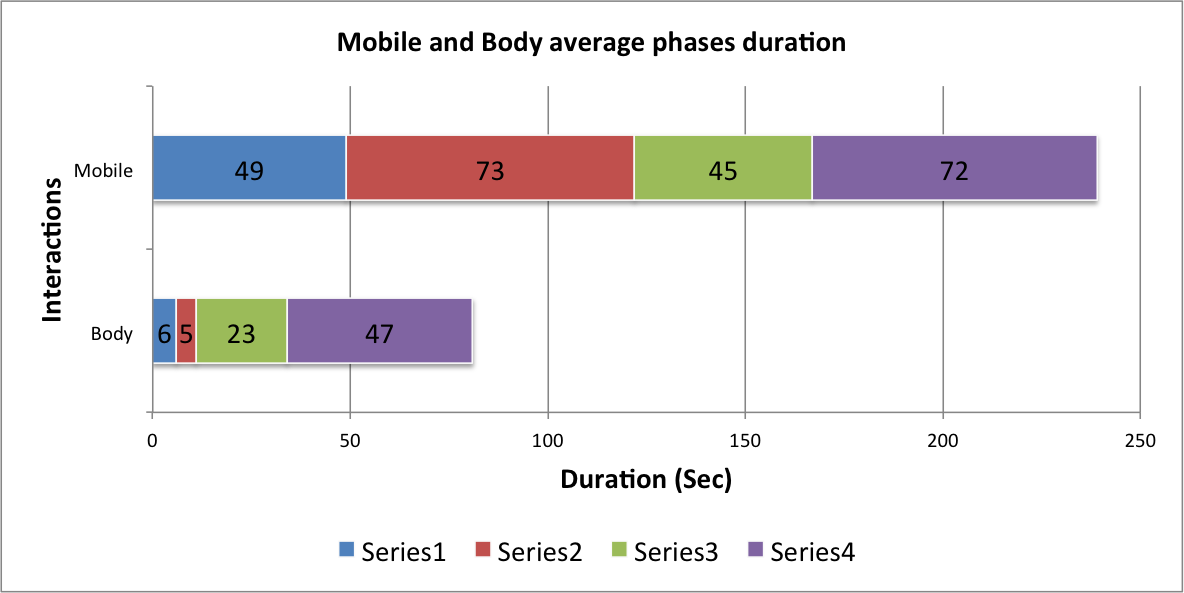
\includegraphics[width=12cm,height=6cm]{Figures/6/mobile_body_performance}%
 \caption{Comparison of body and mobile interaction performance }%
 \label{fig:mobile_body_performance}%
\end{figure}

81 second is the mean value of the all participants with body interaction and 240 seconds is the mean value of the same participants with mobile interaction. The bellow chart shows other comparison of aspects as described.

\begin{figure}[H]
\centering
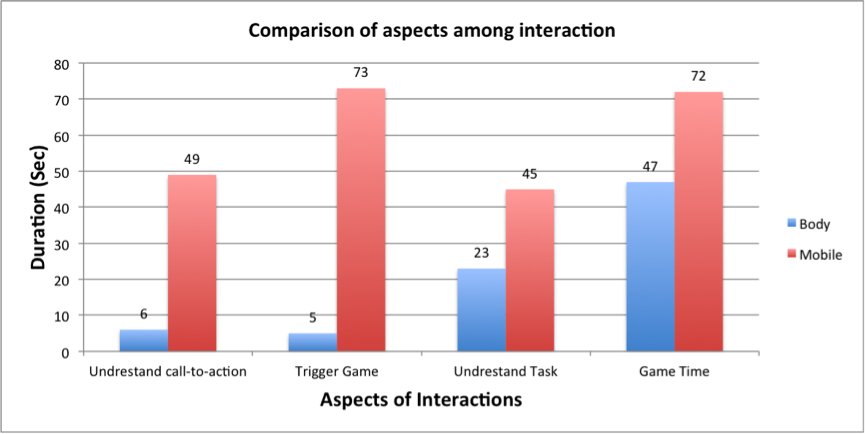
\includegraphics[width=12cm,height=6cm]{Figures/6/mobile_body_aspect}%
 \caption{Comparison of the aspects of interaction among body and mobile }%
 \label{fig:mobile_body_aspect}%
\end{figure}


As can be seen in the chart mobile interaction took much longer than body interaction for each phase or aspects, ANOVA reveals a significant effect of call-to-action of (body vs. mobile)( \emph{(F1,11)=22.4758, p < .001 (p=.0001)}). A post-hoc tukey test shows that participants understood very quickly the call-to-action of body interaction compared to mobile interaction technique, maybe because it is very easy and understandable by any person because of the action ``\emph{to play come near}''is very usual and easy compared to using mobile phone which is not expected at that moment and the users should read and see the information text to understand that requires more cognitive load than simple action of body interaction.

ANOVA reveals a significant difference of triggering game between (body vs. mobile) ( \emph{(F1,11)=124.1066, p < .001}). post-hoc tukey test shows that in body interaction the triggering happens much faster than mobile interaction, This is because mobile technique has many steps to follow in order to trigger the game (like connecting to WiFi, logging to website).


ANOVA reveals a significant difference of task undrestandability between (body vs. mobile) ( \emph{(F1,11)=7.1340, p < .05 (p=.0147)}). A post-hoc tukey test shows that participants undrestand the task very faster compared to mobile technique, one hint could be the body representation itself and in mobile an abstract circle is shown and the interface that takes time to try and error and find what to do.

Interaction time is also significant different as ANOVA test suggests a significant difference between the game interaction ( \emph{(F1,11)=19.7000, p < .001 (p=.01)}) post-hoc tukey test also strongly recommends that body interaction takes less time to complete the interaction comparted to body.

\subsection{Usability issues}
The bellow usability issues are gathered from participant while observing them during the interactions.
\subsubsection{Mobile Interaction}
\begin{enumerate}
\item	Call-to-Action
\begin{enumerate}
\item	At the first glance and moment most participants did not try to read the text on the screen, despite they were expecting other way to get quick information, but after many try with their body they had to read the information text. This could be because of many issues like (amount of text, text size and used icons). And most importantly the text information was being covered by the silhouette, if participants were far the text was readable but when participants would get near to the screen to scan the QR-code or read the IP address, the silhouette drawn by the Kinect camera would occlude part of the information text, which resulted that participants should move a side to scan while facing toward the screen.
\item	Participants did not understand about the phone icon or the browser animation on top of it until they figured by themselves.
\item	IP address was complicated and took time to type in phone.
\item	The size of QR code was small.
\end{enumerate}

\item	Use of mobile phone.
\begin{enumerate}
\item	Participants did not expect at the beginning that they would use their own phone for the interactions; many times participants asked, ``\emph{Should I use my phone?}'' 
\item	Most participants did not read the instruction to tilt their phone and even if they accidently had tilted the phone, it would have not effected because by default the tilt-sensor of the phones were off because of power saving settings. 
\item	There was no instruction to turn-on the tilt-sensor in mobile phone.
\end{enumerate}

\item	Login page
\begin{enumerate}
\item	Some of the participants were confused with the word Login, Participants thought that they would have to provide some sort of username and password to the system, and one participant reacted to this strictly and refused to login to the webpage using his phone.
\end{enumerate}

\item	Task description
\begin{enumerate}
\item	The task description was shown after the participants login to the system despite of whether the phone is tilted or not, Most participants missed to read the task description because they were busy with their phone to tilt it and by that time the description on the screen was gone.
\end{enumerate}

\item	Controller
\begin{enumerate}
\item	Beside small instruction for controller usage but still it was not sufficient because most of the participants did not give time to read it.	
\item	Many participants complained about the elasticity (automatic centering feature) of cursor. They had to reposition the cursor for another location to explore.
\end{enumerate}
\end{enumerate}

\subsubsection {Body Interaction}

\begin{enumerate}
\item	Call-To-Action
\begin{enumerate}
\item	The silhouette is projected in the largest scale for attraction attention but when users trigger the interaction by coming close to the screen then participants could not see themselves, because the silhouette was projected on the top of the screen or sometimes when participants were very close their silhouette was projected on top out of the screen image, This happens because of the mapping of participant location in relation to the screen, if participant moves back then they could see themselves. 
\end{enumerate}

\item	Controller
\begin{enumerate}
\item	Participants tried themselves to find a way to interact, by moving their body; there was no instruction on how to control their silhouette.
\end{enumerate}

\item	Alert image
\begin{enumerate}
\item	Alert image that shows a Hands-Up person lead to confusion at the moment where users were much closer to the system.
\end{enumerate}
\end{enumerate}

\subsubsection{Advertisement video}
\begin{enumerate}
\item The slides were switching fast.
\item Some did not liked the colors and theme. 
\end{enumerate}


\subsection{Advertisement goal}

\subsubsection{Did users understand about advertisement?}

	The criteria for recalling the advertisement was that participants should recall ``\emph{Bauhaus-Walk}'' word and explain what does it do or if the interaction technique gave them an idea what could be the advertisement about, At best users can recall the date, timing and location of the tour program.

\begin{enumerate}

\item	\textbf{Ad goal description} \\
Therefor to find out this, when all participants experienced with the very first interaction technique mobile or body, they were immediately asked about the goal of advertisement, we wanted to know if the participants would understand about the advertisement at their very first try. All of the participants were speaking in English language and the advertisement interaction and the entire participants responded as they finished the interaction. 9 participants accurately described the goal of the advertisement and 2 participants generally described about the goal, the reason behind that was advertisement video, which was shown was in German language, later the video was changed to English for the rest of participants and they responded precisely.

\item	\textbf{Ad-related elements recalled}  \\ 
After the participants described the goal, they were given a piece of sheet to draw and write any element related to the interaction and advertisement with in five minutes. All the sketches drawn and keywords written by the participants were manually analyzed and counted

\begin{figure}[H]
\centering
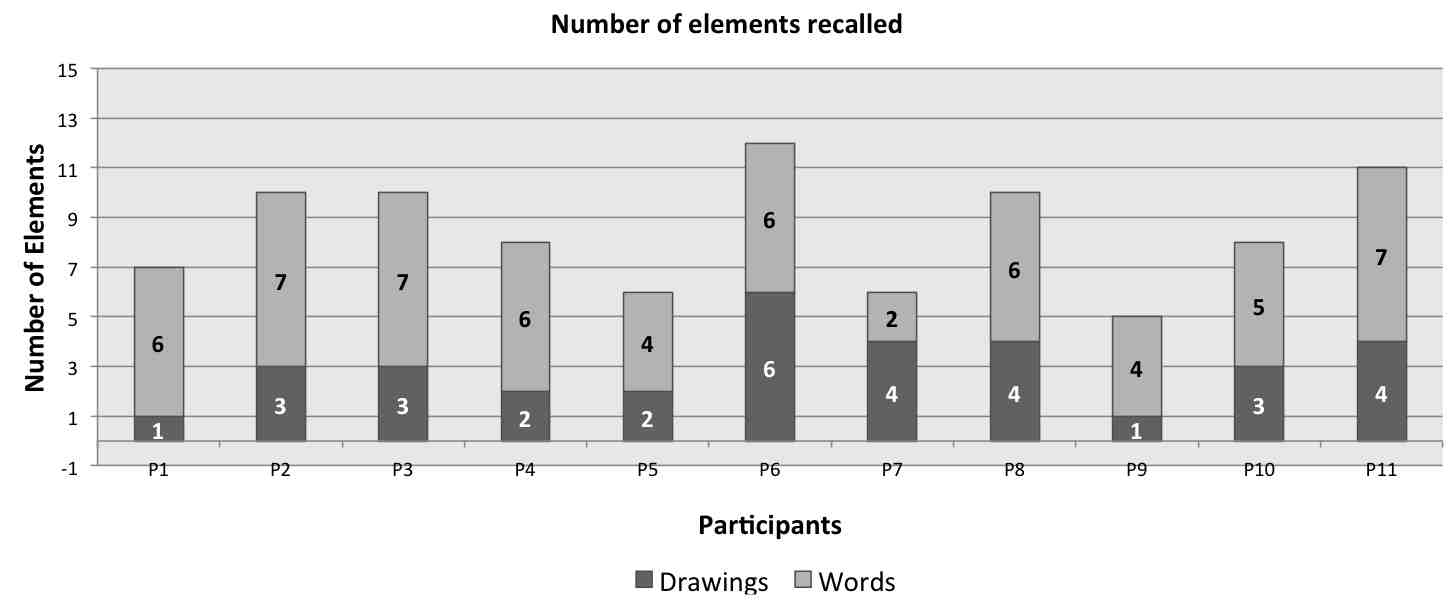
\includegraphics[width=12cm,height=6cm]{Figures/6/word_recall}%
 \caption{Number of words and drawings of the advertisement elements }%
 \label{fig:word_recall}%
\end{figure}

\end{enumerate}

\subsubsection{Word cloud (Wordle)}
All the keywords written in the papers by participants were collected in one text file and using an online tool \cite{wordle} the bellow word cloud was generated.

\begin{figure}[H]
\centering
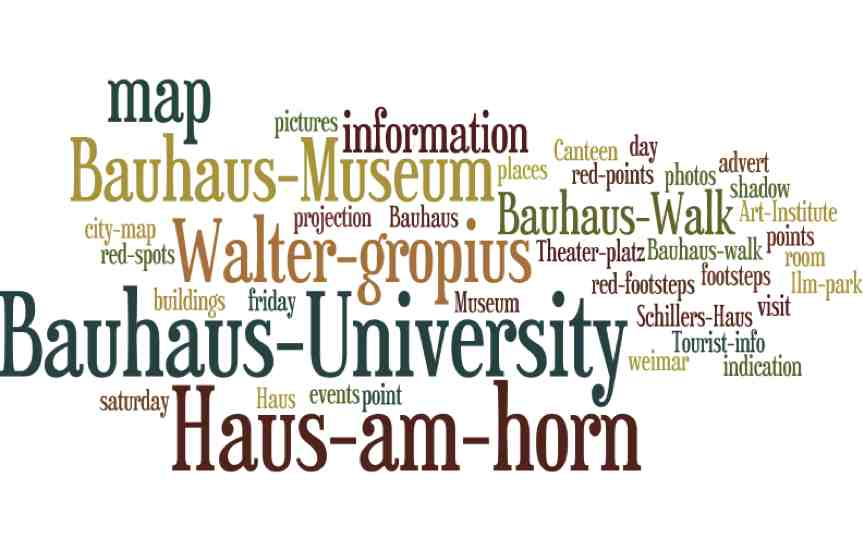
\includegraphics[width=12cm,height=8cm]{Figures/6/wordle}%
 \caption{Word cloud representation of the keywords}%
 \label{fig:wordle}%
\end{figure}

As can be seen, most key words that has high frequency are the ones actually related to the advertisement it seems most location names that participants interacted with are recalled a lot like ``\emph{Bauhaus University}'' ,``\emph{Haus-am-horn}''and others, The program name ``\emph{Bauhaus-Walk}'' is also in high frequency, and even the day of the event is mentioned too.


\subsubsection{Key factors for advertisement understanding}
\begin{enumerate}
\item	\textbf{Game environment} \\
The game environment designed for the interactions had a major impact for understanding the advertisement goal, for example one of the participants replied ``\emph{I saw a map and different places, so I guess touristic places that I can visit in Weimar.}'' Beside the map the blinking points on the map, which more people are familiar that shows interest regions of a city, one participant replied ``\emph{ I think it was about tourist places in the city, at first I saw the map, and there were points on the top}'' By analyzing their reply, they already linked the points with the touristic places.

\item	\textbf{Interaction technique} \\
The interaction technique especially with the body interaction where walking is involved, participants got clue about the advertisement indirectly only by walking and linked walking as visiting locations, like one of the participants replied ``\emph{Discovering Weimar. The Bauhaus-Walk. It was the advertisement about those locations that the people can visit in the tour.}'' It is very fascinating to read that answer from which the whole goal of the advertisement can be derived.

\item	\textbf{Advertisement video} \\
The advertisement video had an impact on the participants to be able to recall the advertisement, one of the participants replied that ``\emph{I saw many pictures coming about Bauhaus and the program times and day}'', despite that the users understood a little about the advertisement they also complained about the video for being fast.

\end{enumerate}


\subsection{Interview Findings}
All the interviews transcripts were coded for better analyzing and finding appropriate connections to categories and these categories are shown as a big diagram attached to appendix B. Each category is discussed separately 

\subsubsection{Mobile Categories}
Many important categories were created from the responder's codes; these categories reflect the functionality, nature, issues and complications of mobile interaction technique. Most of them points out negative concerns and some positive feedbacks too about the interactions, which is discussed bellow.
\begin{enumerate}
\item	\textbf{Comfortable} \\
	Mobile interaction is more comfortable in the context of public environment, users do not feel shy to work with their phone, they have more privacy as one user said ``\emph{I think for people moving in public could be more embarrassing if you just use your phone the people passing by will not pay attention}''. Users can also work with the display from a far location rather than standing in front as one participant said, ``\emph{you can comfortably set far away see the screen and start interacting}''.
\item	\textbf{Activity} \\
	This method has less Activity, participants do not have to move their body to reach certain points in the map, instead they can use their phone and stand or sit steady and with the tip of their finger can easily explore locations, as one of the user said ``\emph{I could go with the tip of my finger and it helped me all the places I visited}''.
\item	\textbf{Dependency}\\
	On the other hand, this interaction is dependent to many things like obviously a mobile phone, if the user does not have a mobile phone the interaction cannot happen, a participant asked, ``\emph{How would I have played if I have not brought my mobile phone?}'' Another dependency is the WIFI connection, one participant pointed out ``\emph{And then the fact that I had to be connected to a WIFI, that was because I did not understand do we have to be in the same Internet (Network)?}'' 

\item	\textbf{Complicated}\\
The process seemed also complicated like first entering the IP-Address or scanning the QR-code, then looking at the instructions and logging with a name, then tilting the phone and finally interacting with the controller elements like the button and cursor, most of the participants complained about this stating like, ``\emph{Because it is a headache for me to take out my phone and use all this login, and waste my time.}'' another commented like ``\emph{for exploring you have to push that red button, that was a bit confusing.}''


\item	\textbf{Annoying}\\
One of the annoying things pointed out by the participant was the QR-Code was being covered by the person silhouette standing in front of the display the user said ``\emph{QR-Code was small and when I was coming near the screen to scan the code, my body was covering it}''.

\item	\textbf{Clarity}\\
There were many instructions like Access-information, mobile instruction and task instruction, but these instruction was also not clear to them as one of the participant mentioned, ``\emph{that controller was also not clear, because I though the red areas is the touch area that I can scroll and the red button was a click}'' another participant replied like ``\emph{there were very few descriptions, I guess the word login was miss-phrased, it was not really a login it was just chose a name}''. Another participant was not sure if to use mobile phone or the screen has touch capability as he replied ``\emph{at first I saw the map, and there were points on the top first I tried to touch}''.


\end{enumerate}


\subsubsection{Body Categories}
Body interaction was more appreciated by the participants; from the interview transcripts the bellow positive and negative opinions were derived and categorized.

\begin{enumerate}
\item	\textbf{Enjoyment}\\
Participants had the sense of enjoyment and fun, as one of participants said, ``\emph{I liked the second one because it seemed more involving and I think it was more fun}'', another user said ``\emph{I liked this interaction; it was more good and fun.}'' , 

\item	\textbf{Easy}\\
Users found the interaction to be very easy, simple and smooth, a user said, ``\emph{The body movement was good it was smooth}'' another user said, ``\emph{It was much easier than the previous one, it was much better, umm it was not confusing}''. The call-to-Action seemed much easier, one user said, ``\emph{I saw saying me to come near, and when I came the game started, that was very easy to use}'', and the interaction with the game elements was also easy to understand, one participants said ``\emph{it was easy to come near to the screen and first I did not understand how to play the game but when I saw my avatar that is moving with me then I realized and did the tasks}''

\item	\textbf{Immersion}\\
Some participants said they were some how immersed with the game, like one said, ``\emph{I felt that I was really part of it}'', another said, ``\emph{With the body you look your own avatar in the map and you feel that you are in the map.}''

\item	\textbf{Engaging}\\
The body technique seemed also very engaging and users wanted to play more and more, one said, ``\emph{It is so engaging and it is like that it needs you}'', another said, ``\emph{it is like you want to put the footsteps exactly on the street}'' , ``\emph{it seemed more involving}''. 

\item	\textbf{Issues}\\
On the other hand, body interaction had also some issues, like one of the participants pointed out that the interaction would be difficult if it is in crowded area, one said, ``\emph{If two people interact then they can crash at each other}''. Participants complained about physical space ``\emph{I felt was the space there was not enough space in here}''. Bad tracking of the body and unexpected locations were triggered by fast movement like, one participants said, ``\emph{I guess the application was tracking me really bad}'', ``\emph{when I was moving to some areas fast suddenly that point was being triggered.}''

\item	\textbf{Embarrassing}\\
Some participants said that they would not try at public because it could be shame or embarrassment for their selves, ?moving in public could be more embarrassing?

\item	\textbf{Confusion}\\
The projection of silhouette on the advertisement also made some participants confused and that was also distractive, like one said, ``\emph{I saw my silhouette at the last time I was playing, because I was curious that why is it there}''. 

\end{enumerate}


\subsubsection{Advertisement}

\begin{enumerate}
\item	\textbf{Interface}\\
The interface was appreciated by all the participants, as one said, ``\emph{I really liked the map}'', another user said, ``\emph{the footsteps were cute}''.

\item	\textbf{Non-controllability}\\
The flow of the interaction was also observed by the users, which they found annoying like, one participants noticed that ``\emph{I do not want to be forced to see all the places and then see the advertisement}'', the video advertisement was also not in the control a user said, ``\emph{There was nothing to answer, it gave me the impression that okay; this was an advertisement someone did it and I could not change the flow of it.}'' 

\item	\textbf{Distraction}\\
The projection of silhouette after the interaction body or mobile technique was a distraction factor, because participants would not notice the video advertisement but would notice themselves. 

\item	\textbf{Speed}\\
The pictures for the locations and the advertisement video were fast, a user said, ``\emph{The description of the places were very fast, when I was trying to read it, it disappeared.}'', 
\end{enumerate}

\subsection{Application Performance}
Application performed quite well for both single and multi-user interactions, Application did not crashed nor hanged in the middle of interaction. In multi-user interaction, application faced some delay in both body and mobile because of many participants 5-7 at the same time, this issue got solved by changing the 
JRE version 32bit to JRE version 64bit and along with this the processing version was also changed from 32bit to 64bit and increased the maximum usage memory to highest in processing.


\begin{figure}[H]
    \centering
    \begin{subfigure}[H]{0.45\textwidth}
        \centering
        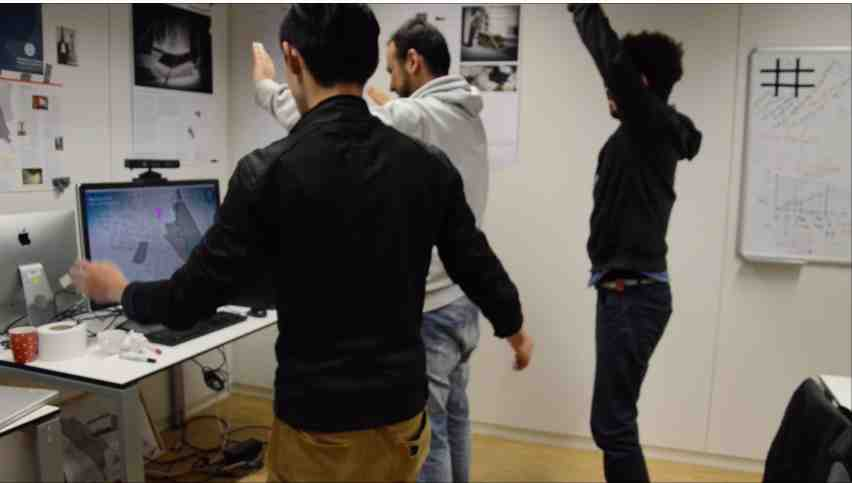
\includegraphics[width=\textwidth,height=4cm]{Figures/6/groupBody}
        \caption{Group body interaction.}
        \label{fig:groupbody}
    \end{subfigure}
    \hfill
    \begin{subfigure}[H]{0.45\textwidth}
        \centering
        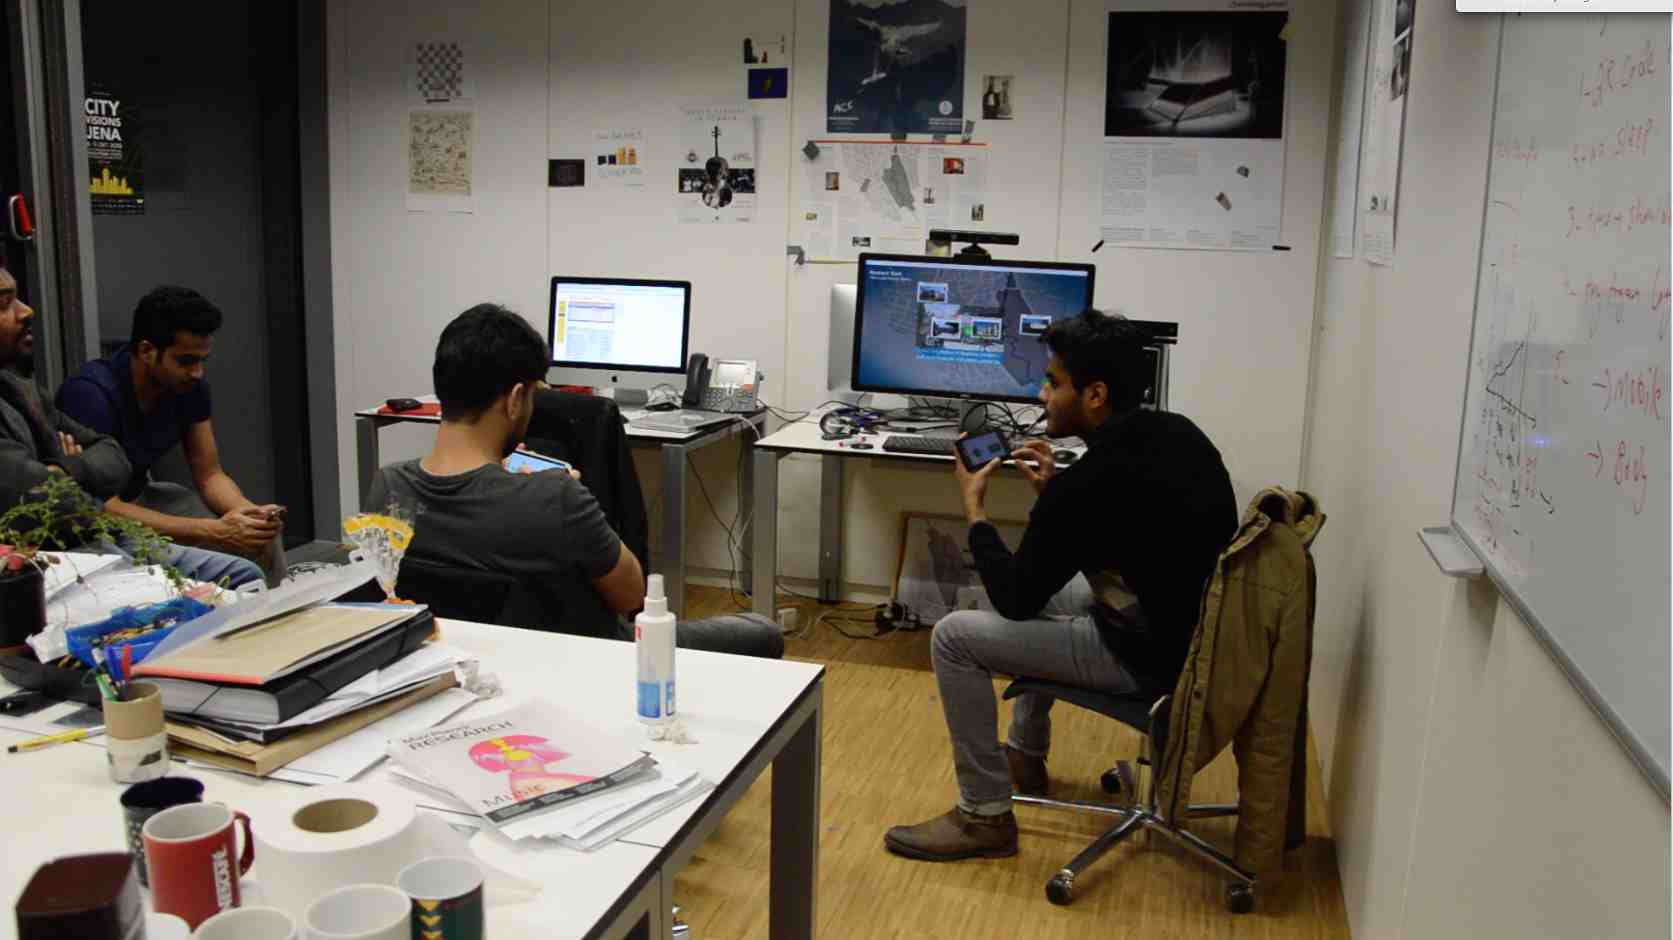
\includegraphics[width=\textwidth,height=4cm]{Figures/6/groupMobile}
        \caption{Group mobile interaction.}
        \label{fig:groupmobile}
    \end{subfigure}
    \caption{}
    \label{fig:Focus_group_room_interactive}
\end{figure}


\section{Conclusion}
This chapter concludes that with body interaction technique, participants felt more satisfied than mobile technique and preferred the use of body than mobile in public environment.

Learnability of body interaction was better than mobile interaction, because of the problems mentioned like (unclear access-info text, unfamiliarity with QR code or phone icons, Registration) and many other things that made the process quite complicated whereas the body interaction had none of them.The efficiency of accessing the system was also significant between body interaction and mobile interaction, because of the lengthy process, which was required for mobile interaction, which made it really hard for participants.
Body representation on the map provides a strong clue of “walking” which was the main task and the learnability of task was very significant compared to mobile technique, which showed a circle colored shape, along the understandability task completion time was also significant, participants completed the task much earlier than mobile technique. 
Along the usability issues most of the participants understood the goal and purpose of advertisement in both techniques.

Considering the above issues, the next step would be to refine both prototypes and make it ready for evaluation on public space.













